\documentclass[10pt,a4paper]{article}
\usepackage[margin=18mm]{geometry}
\usepackage{amsmath,amssymb,graphicx,booktabs,tikz,pgfplots,enumitem,titlesec}
\pgfplotsset{compat=1.18}\usetikzlibrary{arrows.meta}
\setlength{\parindent}{0pt}\setlength{\parskip}{3pt}
\setlist[itemize]{nosep,topsep=2pt,leftmargin=*}
\titlespacing*{\section}{0pt}{7pt}{4pt}\titlespacing*{\subsection}{0pt}{5pt}{3pt}
\begin{document}
\begin{center}{\large\bfseries SC4001 -- Part B: Chest X-ray Classification}\\Hu Han \quad U2320036H\end{center}

\textbf{Generative AI Declaration:}

I used \textbf{Codex} to assist with the generation of selected code segments during the development of this assignment. The tool was used primarily to generate initial code templates and to obtain suggestions for implementing specific programming tasks. All AI-generated code was carefully reviewed, modified where necessary, integrated into the overall solution by me, and tested to ensure it met the assignment requirements. I verified the correctness of the generated code through manual inspection, compilation/execution testing, debugging, and comparison with the assignment specifications and relevant course materials. The final submitted work represents my own understanding and effort. I take full responsibility for the accuracy, functionality, and academic integrity of the submitted solution.

\textbf{Generative AI Tool Used:} Codex

\textbf{Purpose of Use:} Code generation and programming assistance

\textbf{Verification Method:} Manual code review, testing, debugging, and validation against assignment requirements

\section*{B1}
\subsection*{(a) Validation Loss and Accuracy Curve for Each Learning Rate}
\begin{center}
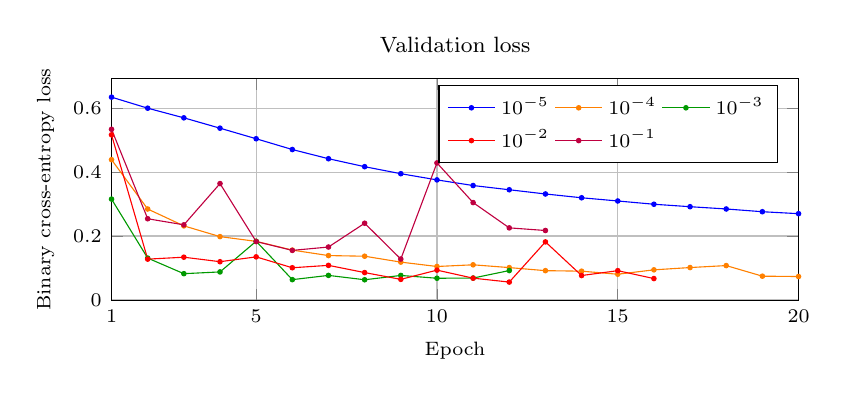
\begin{tikzpicture}
\begin{axis}[width=0.85\linewidth,height=4.4cm,
title={Validation loss},ylabel={Binary cross-entropy loss},
xlabel={Epoch},xmin=1,xmax=20,xtick={1,5,10,15,20},
tick label style={font=\scriptsize},label style={font=\scriptsize},
title style={font=\footnotesize},legend style={font=\scriptsize,legend columns=3},
legend pos=north east,grid=major]
\addplot[blue,mark=*,mark size=0.8pt] coordinates {(1,0.63451133) (2,0.59996149) (3,0.56974258) (4,0.53735279) (5,0.50429701) (6,0.47055277) (7,0.44180545) (8,0.41685113) (9,0.39488831) (10,0.37553643) (11,0.35786439) (12,0.34466402) (13,0.33144872) (14,0.31957336) (15,0.30954381) (16,0.29928590) (17,0.29159426) (18,0.28450631) (19,0.27587533) (20,0.26980339)};\addlegendentry{$10^{-5}$}
\addplot[orange,mark=*,mark size=0.8pt] coordinates {(1,0.43876368) (2,0.28436528) (3,0.23160893) (4,0.19799902) (5,0.18307286) (6,0.15577123) (7,0.13865984) (8,0.13664370) (9,0.11815369) (10,0.10447863) (11,0.10975297) (12,0.10101492) (13,0.09143878) (14,0.08980383) (15,0.08025142) (16,0.09398730) (17,0.10117186) (18,0.10730940) (19,0.07416265) (20,0.07307998)};\addlegendentry{$10^{-4}$}
\addplot[green!60!black,mark=*,mark size=0.8pt] coordinates {(1,0.31537276) (2,0.13073009) (3,0.08196583) (4,0.08747035) (5,0.18343685) (6,0.06329508) (7,0.07660278) (8,0.06294419) (9,0.07641585) (10,0.06768110) (11,0.06829708) (12,0.09173201)};\addlegendentry{$10^{-3}$}
\addplot[red,mark=*,mark size=0.8pt] coordinates {(1,0.51658575) (2,0.12749663) (3,0.13355427) (4,0.11944834) (5,0.13458741) (6,0.10051212) (7,0.10801720) (8,0.08538790) (9,0.06419832) (10,0.09307003) (11,0.06794226) (12,0.05568889) (13,0.18149090) (14,0.07617711) (15,0.09137616) (16,0.06669246)};\addlegendentry{$10^{-2}$}
\addplot[purple,mark=*,mark size=0.8pt] coordinates {(1,0.53387402) (2,0.25390384) (3,0.23484317) (4,0.36396147) (5,0.18260246) (6,0.15492083) (7,0.16539761) (8,0.23984433) (9,0.12778933) (10,0.42855946) (11,0.30452543) (12,0.22536111) (13,0.21710801)};\addlegendentry{$10^{-1}$}
\end{axis}
\end{tikzpicture}
\end{center}
\begin{center}
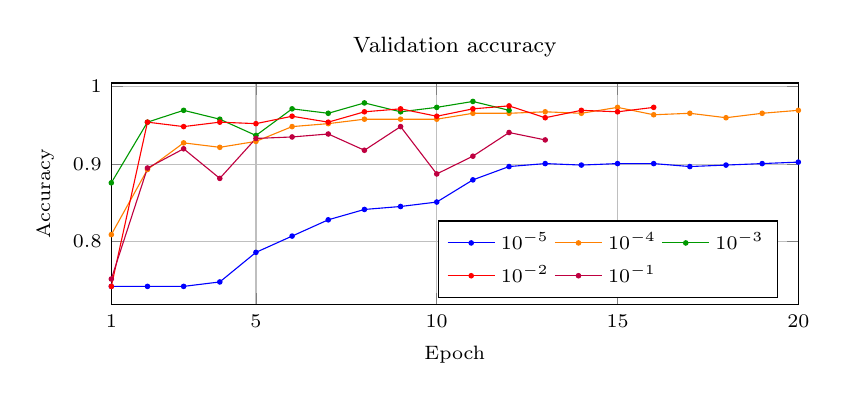
\begin{tikzpicture}
\begin{axis}[width=0.85\linewidth,height=4.4cm,
title={Validation accuracy},ylabel={Accuracy},
xlabel={Epoch},xmin=1,xmax=20,xtick={1,5,10,15,20},
tick label style={font=\scriptsize},label style={font=\scriptsize},
title style={font=\footnotesize},legend style={font=\scriptsize,legend columns=3},
legend pos=south east,grid=major]
\addplot[blue,mark=*,mark size=0.8pt] coordinates {(1,0.74236641) (2,0.74236641) (3,0.74236641) (4,0.74809160) (5,0.78625954) (6,0.80725191) (7,0.82824427) (8,0.84160305) (9,0.84541985) (10,0.85114504) (11,0.87977099) (12,0.89694656) (13,0.90076336) (14,0.89885496) (15,0.90076336) (16,0.90076336) (17,0.89694656) (18,0.89885496) (19,0.90076336) (20,0.90267176)};\addlegendentry{$10^{-5}$}
\addplot[orange,mark=*,mark size=0.8pt] coordinates {(1,0.80916031) (2,0.89312977) (3,0.92748092) (4,0.92175573) (5,0.92938931) (6,0.94847328) (7,0.95229008) (8,0.95801527) (9,0.95801527) (10,0.95801527) (11,0.96564885) (12,0.96564885) (13,0.96755725) (14,0.96564885) (15,0.97328244) (16,0.96374046) (17,0.96564885) (18,0.95992366) (19,0.96564885) (20,0.96946565)};\addlegendentry{$10^{-4}$}
\addplot[green!60!black,mark=*,mark size=0.8pt] coordinates {(1,0.87595420) (2,0.95419847) (3,0.96946565) (4,0.95801527) (5,0.93702290) (6,0.97137405) (7,0.96564885) (8,0.97900763) (9,0.96755725) (10,0.97328244) (11,0.98091603) (12,0.96946565)};\addlegendentry{$10^{-3}$}
\addplot[red,mark=*,mark size=0.8pt] coordinates {(1,0.74236641) (2,0.95419847) (3,0.94847328) (4,0.95419847) (5,0.95229008) (6,0.96183206) (7,0.95419847) (8,0.96755725) (9,0.97137405) (10,0.96183206) (11,0.97137405) (12,0.97519084) (13,0.95992366) (14,0.96946565) (15,0.96755725) (16,0.97328244)};\addlegendentry{$10^{-2}$}
\addplot[purple,mark=*,mark size=0.8pt] coordinates {(1,0.75190840) (2,0.89503817) (3,0.91984733) (4,0.88167939) (5,0.93320611) (6,0.93511450) (7,0.93893130) (8,0.91793893) (9,0.94847328) (10,0.88740458) (11,0.91030534) (12,0.94083969) (13,0.93129771)};\addlegendentry{$10^{-1}$}
\end{axis}
\end{tikzpicture}
\end{center}

\subsection*{(b) Learning Rate Comparison Table}

Pneumonia is positive (label 1); the prediction threshold is 0.5. $TP,TN,FP,FN$ denote true positives, true negatives, false positives and false negatives; $N=TP+TN+FP+FN$.
\[
\begin{aligned}
\mathrm{Accuracy} &= \frac{TP+TN}{N}, &
\mathrm{Error} &= 1-\mathrm{Accuracy},\\
\mathrm{Sensitivity} &= \frac{TP}{TP+FN}, &
\mathrm{Specificity} &= \frac{TN}{TN+FP}.
\end{aligned}
\]
Validation loss is binary cross-entropy, with true label $y_i$ and predicted pneumonia probability $p_i$:
\[
\mathcal{L}_{\mathrm{val}}=-\frac{1}{N}\sum_{i=1}^{N}
\bigl[y_i\log p_i+(1-y_i)\log(1-p_i)\bigr].
\]
Each row reports the minimum-error checkpoint (ties: lower loss, then earlier epoch). Error, sensitivity and specificity are percentages.

\begin{center}\small
\begin{tabular}{rrrrrrr}\toprule
Learning rate & Best epoch & Epochs run & Val. loss & Error (\%) & Sens. (\%) & Spec. (\%)\\\midrule
$10^{-5}$ & 20 & 20 & 0.2698 & 9.73 & 96.14 & 73.33 \\
$10^{-4}$ & 15 & 20 & 0.0803 & 2.67 & 97.69 & 96.30 \\
$10^{-3}$ & 11 & 12 & 0.0683 & 1.91 & 97.94 & 98.52 \\
$10^{-2}$ & 12 & 16 & 0.0557 & 2.48 & 98.20 & 95.56 \\
$10^{-1}$ & 9 & 13 & 0.1278 & 5.15 & 96.92 & 88.89 \\
\bottomrule\end{tabular}
\end{center}
\subsection*{(c) Optimal Learning Rate and Discussion}
Optimal learning rate is $10^{-3}$ with the lowest validation error of $1.91\%$.
The learning curves show that the model with learning rate $10^{-3}$ converges faster than other learning rates, with the best validation loss and accuracy in most of the epochs.
Sensitivity and specificity are also needed to interpret model performance because they reflect the models’ ability to detect pneumonia cases and correctly identify healthy subjects, respectively.
And the learning rate $10^{-3}$ has high sensitivity and specificity, proving its effectiveness in accurate detection of both categories.
\subsection*{(d) Test Performance}

\section*{B2}
\subsection*{(a) VGG-like Architecture and Training}
\subsection*{(b) Validation Curves and Batch Size Comparison}
\subsection*{(c) Optimal Batch Size and Discussion}
\subsection*{(d) Test Performance}

\section*{B3}
\subsection*{(a) ResNet-like Architecture and Training}
\subsection*{(b) Model Performance}
\subsection*{(c) Architecture Comparison and Discussion}

\section*{B4}
\subsection*{(a) X-ray Selection and Grad-CAM Implementation}
\subsection*{(b) Grad-CAM Overlays}
\subsection*{(c) Comparison and Interpretation}

\end{document}
